\def\QRCODE{TB_IPR_TUT.IMG.point_processes_generation_matlabqrcode.png}
\def\QRPAGE{http://www.iptutorials.science/tree/master/TB_IPR/TUT.IMG.point_processes_generation/matlab}
\mcorrectionsection{Matlab correction}

\subsection{Poisson and other classical processes}
To generate a conditional Poisson process, the following command is used:
\begin{matlab}
n=200;
[x, y] = semi_alea(n, 0, 0, 100, 100);
plot(x,y,'*');title('Conditional Poisson process');
axis square
\end{matlab}
The simulation window is given as a parameter, as well as the number of points. This is illustrated in Fig.\iflabelexists{fig:spatialpp:enonce:ppp}{\ref{fig:spatialpp:enonce:ppp}}{\ref{fig:matlab:spatialpp:ppp}.

\begin{figure}[htbp]
 \centering
 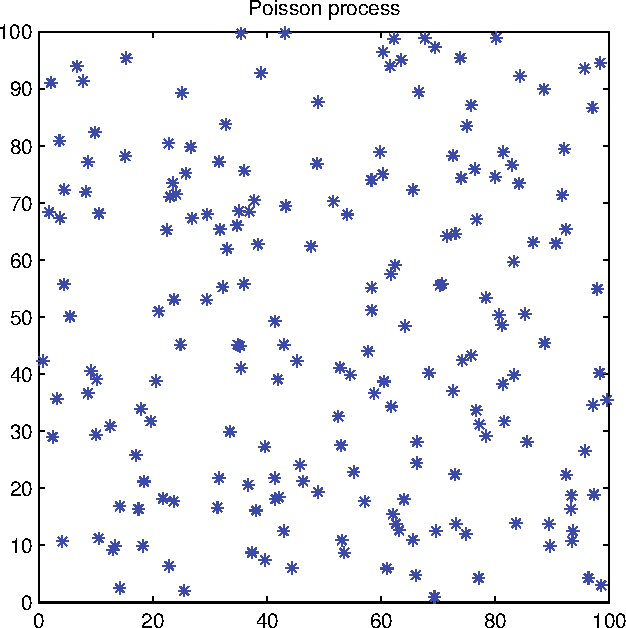
\includegraphics[width=5cm]{poissonprocess.pdf}
 \caption{Poisson point process}
 \label{fig:matlab:spatialpp:ppp}
\end{figure}}

\begin{matlab}
function [x,y]=semi_alea(point_nb,xmin,xmax,ymin,ymax)
% Conditional Poisson Point process
% uniform distribution
% point_nb is the number of points
% xmin, xmax, ymin, ymax define the domain
x = xmin + (xmax-xmin)*rand(point_nb, 1);
y = ymin + (ymax-ymin)*rand(point_nb, 1);
\end{matlab}



To generate a point cloud normally distributed around the point $(a,b)$, one can use the Matlab function \minline{randn}. This is illustrated in Fig.\ref{fig:matlab:spatialpp:npp}.

\begin{matlab}
% Normal distribution, centered around (a,b)
a=0;
b=0;
x = a + 50 * randn(200,1);
y = b + 50 * randn(200,1);
figure();
plot(x, y, '*');title('Std normal distribution');
axis square
\end{matlab}


\begin{figure}[htbp]
 \centering
 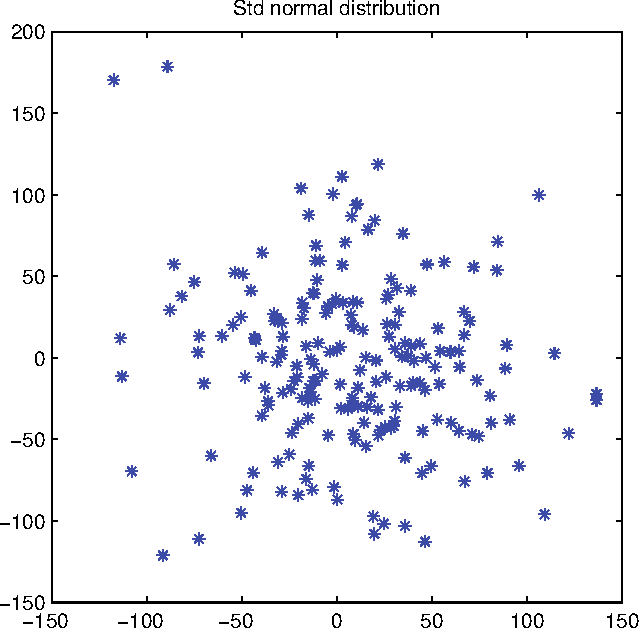
\includegraphics[width=5cm]{stdnormalprocess.pdf}
 \caption{Normal standard distribution of the point process around coordinates $(0,0)$.}
 \label{fig:matlab:spatialpp:npp}
\end{figure}


\subsection{Neyman-Scott processes}
The Neyman-Scott process is a way of simulating clustered processes located around root points issued from a root point process.

\begin{matlab}
function [x,y]=semi_NS(nRoot, xmin, xmax, ymin, ymax, lambdaS, rSon)
% Neyman-Scott process simulation
% i.e. aggregate of processes
% nRoot   : number of agregates
% lambdaS : number of points, lambda is a density, S is the spatial support area
% rSon    : radius around agregate (points are distributed in a square)

% should generate the number of sons
n = poissrnd(lambdaS, nRoot, 1);

% Allocation of memory
nb = sum(n(:));
x=zeros(nb,1);
y=zeros(nb,1);

indice=1;
% loop over all agregates
for i=1:nRoot
    xr=xmin+randi(xmax-xmin); % root point
    yr=ymin+randi(ymax-ymin);
    for j=1:n(i)
        dx=randi(2*rSon)-rSon;
        dy=randi(2*rSon)-rSon;
        
        x(indice)=xr+dx;
        y(indice)=yr+dy;
        indice = indice + 1;
    end
end
\end{matlab}

The result is given by the following command and illustrated in 
\iflabelexists{fig:point_process_generation:neymanscott}{Fig.\ref{fig:point_process_generation:neymanscott}.}{Fig.\ref{fig:neymanscott}.
\begin{figure}
 \centering
 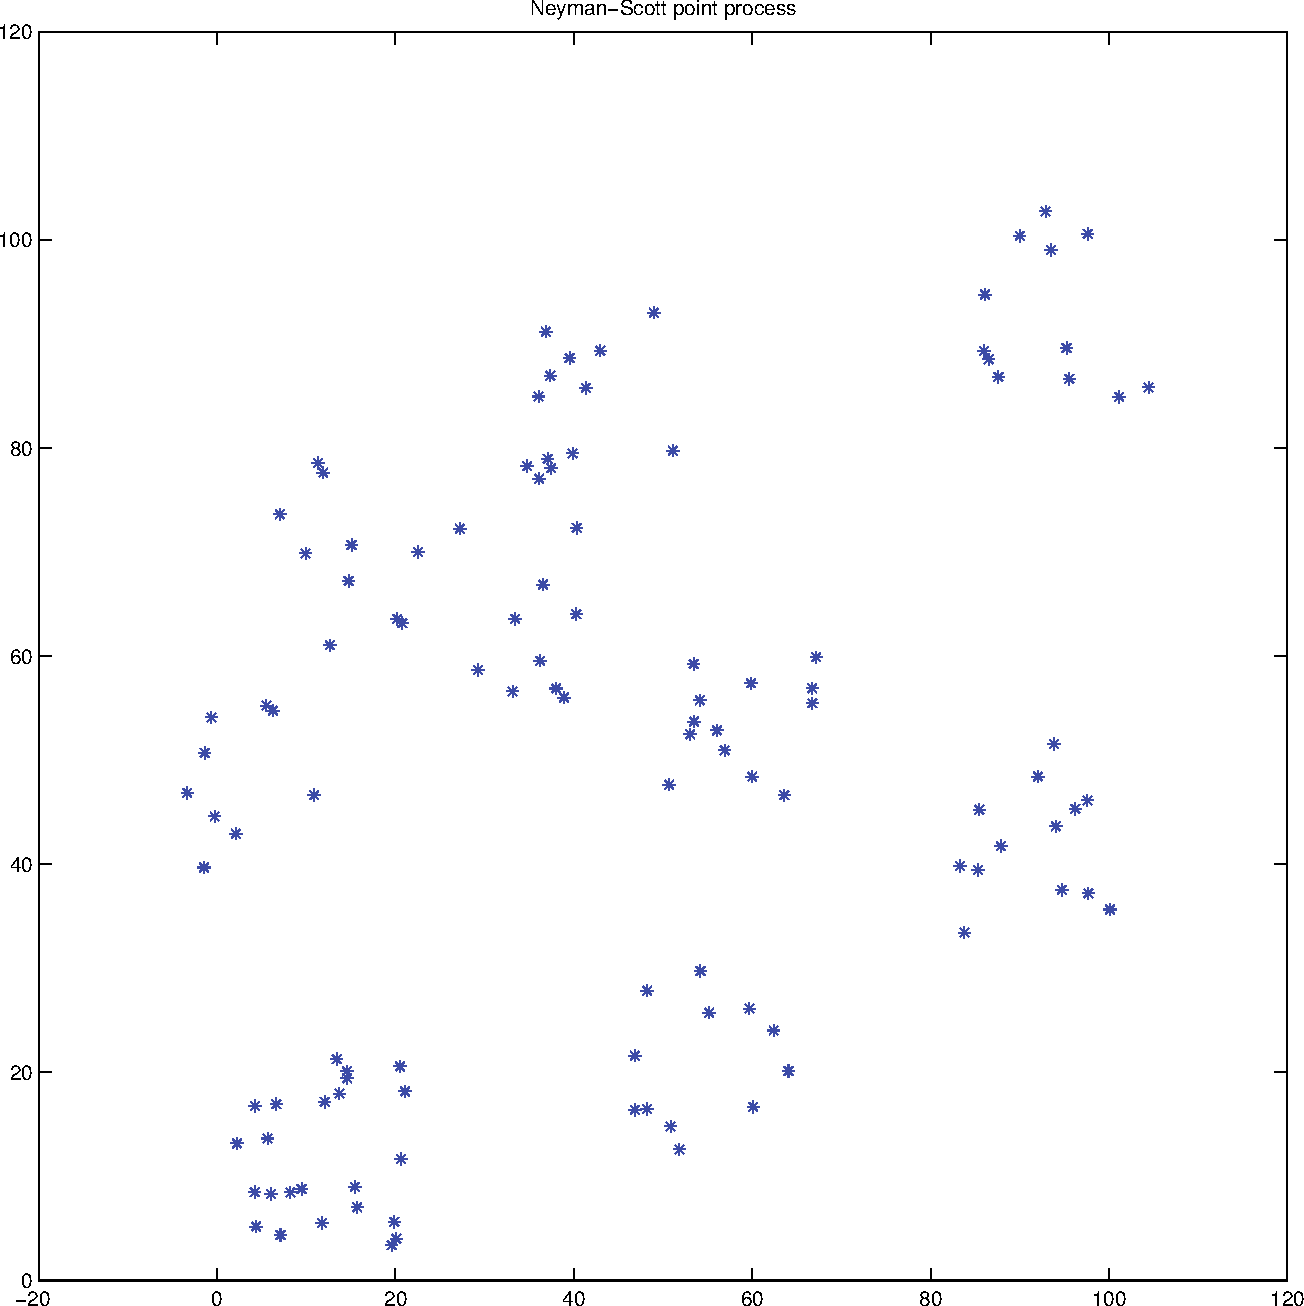
\includegraphics[width=6cm]{neymanscottprocess.pdf}
 \caption{Neyman-Scott point process with $h_{child}=10$ and $n_{par}=10$.}
 \label{fig:neymanscott}
\end{figure}
} % iflabelexists

\begin{matlab}
[x,y]=semi_NS(3,0,100,0,100,20,10);
plot(x,y,'*');title('Neyman-Scott point process');
\end{matlab}

\subsection{Gibbs point processes}
The Gibbs point process uses the definition of an energy in order to attract or repulse points.
First of all, the energy function is coded with the following function \minline{stairsEnergy}. Its results are illustrated in Fig.\ref{fig:point_process_generation:matlab:energyfunction}.
\begin{figure}[ htbp ]
 \centering
 \subfloat[Energy function $f$ for regular distribution.]{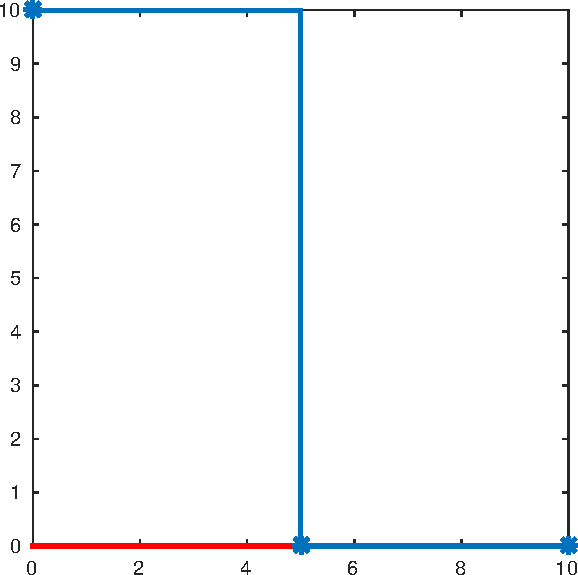
\includegraphics[width=.3\linewidth]{energyfunction.pdf}}\hfill
 \subfloat[Energy function $f$ for agregated distribution.]{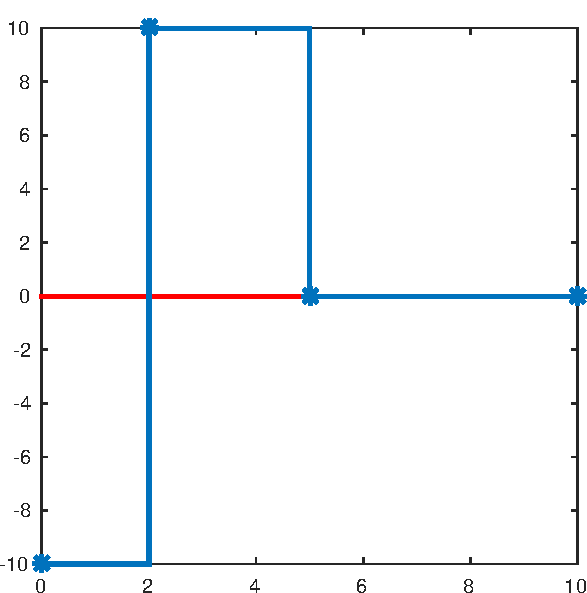
\includegraphics[width=.3\linewidth]{energyfunction2.pdf}}\hfill
 \subfloat[Energy function $f$ for agregated distribution.]{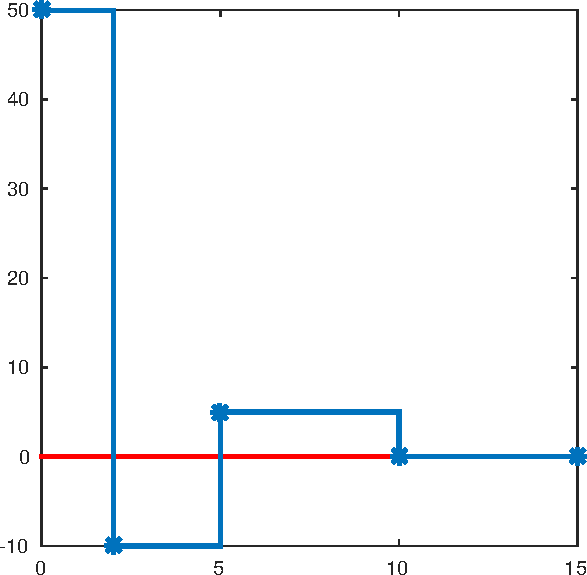
\includegraphics[width=.3\linewidth]{energyfunction3.pdf}}
 \caption{Different energy functions.}
 \label{fig:point_process_generation:matlab:energyfunction}
\end{figure}

The following code ise used to evaluate the energy. The different steps are passed as arrays of values.
\begin{matlab}
function e = stairsEnergy(distance, steps, energy)
% This function returns e with same size as distance.
% e takes the value given in variable energy according to the steps
% distance: vector of all distances between points
% steps   : steps for energy function (unit: distance)
% energy  : value of energy for each step
e = zeros(size(distance));

prev_step = 0;
for i=1:length(steps)
    e(distance>=prev_step & distance<steps(i)) = energy(i);
    prev_step=steps(i);
end
\end{matlab}

To generate the Gibbs process, the following code can be used. It is illustrated in 
Fig.\ref{fig:point_process_generation:matlab:gibbs}.
\begin{matlab}
figure
subplot(241)
[x1,y1]=semi_alea(100,0,100,0,100);
plot(x1,y1,'*');title('Poisson point process');
axis square

subplot(242)
steps = [0,5,10];
energy= [10,0,0];
functionEnergy = @(x)stairsEnergy(x,steps, energy);
[x2,y2]=semis_inter(100,0,100,0,100,2000, functionEnergy);
plot(x2,y2,'*');title('Gibbs point process: regular');
axis square
subplot(246)
plot(0:10,zeros(1,11),'r','linewidth',2);hold on; 
stairs(steps, energy,'*-','linewidth',2);title('Energy function')
axis square

subplot(243)
steps = [0,2,5,10];
energy= [-10,10,0,0];
functionEnergy = @(x)stairsEnergy(x,steps, energy);
[x3,y3]=semis_inter(200,0,100,0,100,200, functionEnergy);
plot(x3,y3,'*');title('Gibbs point process: agregated');
axis square
subplot(247)
plot(0:10,zeros(1,11),'r','linewidth',2);hold on;
stairs(steps,energy,'*-','linewidth',2); title('Energy function')
axis square

subplot(244)
steps = [0,2,5,10,15];
energy= [50,-10,5,0,0];
functionEnergy = @(x)stairsEnergy(x,steps, energy);
[x4,y4]=semis_inter(100,0,100,0,100,200, functionEnergy);
plot(x4,y4,'*');title('Gibbs point process: agregated');
axis square
subplot(248)
plot(0:10,zeros(1,11),'r','linewidth',2);hold on;
stairs(steps, energy,'*-','linewidth',2); title('Energy function')
axis square
\end{matlab}

\begin{figure}[htbp]
\centering
\subfloat[Regular distribution.]{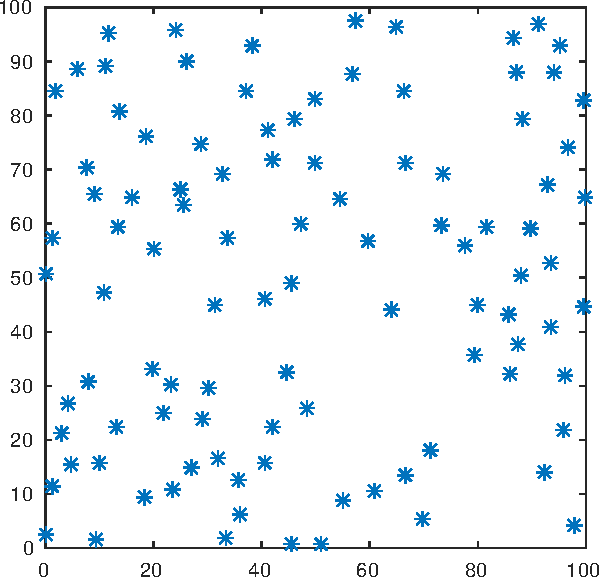
\includegraphics[width=.3\linewidth]{gibbs_regular}}\hfill
\subfloat[Agregated distribution.]{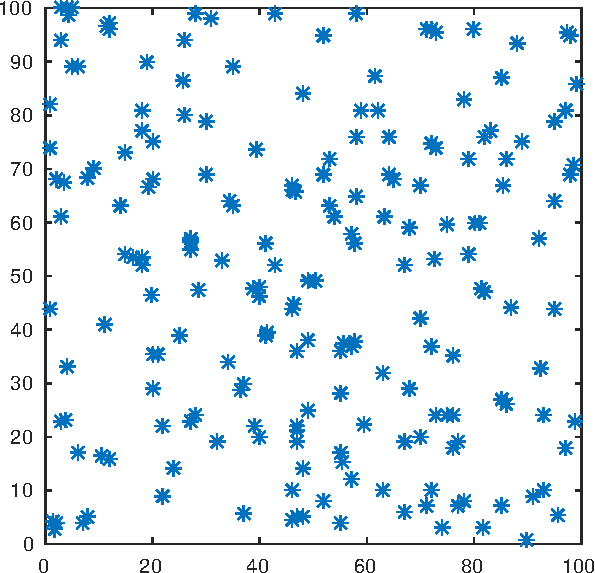
\includegraphics[width=.3\linewidth]{gibbs_agregated2}}\hfill
\subfloat[Agregated distribution.]{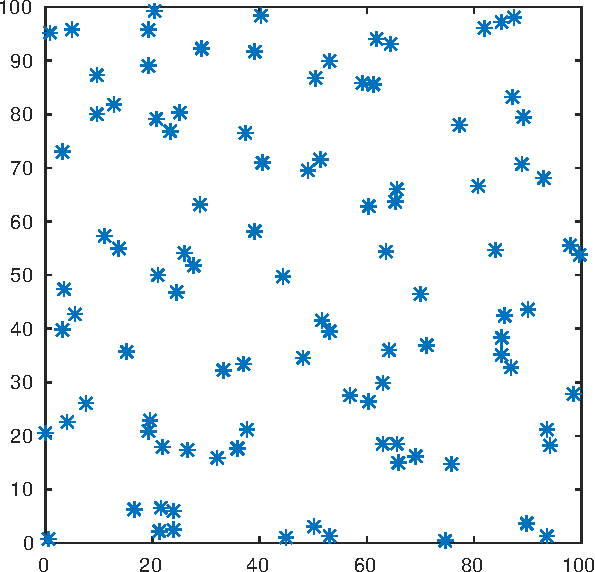
\includegraphics[width=.3\linewidth]{gibbs_agregated3}}
\caption{Gibbs process with different energy functions.}
\label{fig:point_process_generation:matlab:gibbs}
\end{figure}

The principle of the algorithm is to iteratively add one point that minimizes the energy after several trials. In order to speed up the process, notice that only one point is moved, and it is thus sufficient to only compute the distances from this point to all others.

\begin{matlab}
function [x,y]=semis_inter(point_nb, xmin,xmax, ymin,ymax, nbiter, energyFunction)
% simulation of a Gibbs point process
% point_nb is the number of points to plot
% xmin and xmax define the X domain of points
% ymin and ymax define the Y domain of points
% nbiter is the number of iterations, i.e. the number of times a point will be given a try to move
%
% energyFunction is an optional argument defining a function that takes a distance as a parameter and returns an energy (see example at the end of this code, with the default value of this function).
if nargin < 7
    energyFunction = @exampleEnergyFunction;
end

rng(0)
% Start with a poisson point process
[x,y]=semi_alea(point_nb,xmin,xmax,ymin,ymax);
%plot(x, y, 'b*'); hold on
% The variable indices is used to select a point
indices = 1:length(x);

for i=1:nbiter
    % choose a random point among previous process
    j=randi(length(x));
        
    % all points except jth
    x2 = x(indices~=j);
    y2 = y(indices~=j);
    
    % compute the energy associated to the point j
    e1 = energyFromPoint(energyFunction, x, y, x(j), y(j));
    
    % try to minimize energy with new points
    for m=1:10
        % new point 
        [xx,yy] = semi_alea(1, xmin, xmax, ymin, ymax);
        
        e2 = energyFromPoint(energyFunction, x2, y2, xx, yy);
        % the new point is kept if energy is less than previous configuration
        if e2<e1
            x(j)=xx;
            y(j)=yy;
            e1=e2;
        end 
    end
end % end for
end % end function
\end{matlab}

The next functions evaluate the total energy of the point process. The main argument is the set of all distances $D$ between all pairs of points.
\begin{matlab}
function e = energy(energyFunction, D, k)
% compute the energy between all the distances D and the point k
%
% if xx and yy are provided, this new point tries to replace the jth point
dist = sqrt(D(k,:).^2); % Euclidean distance
ee = energyFunction(dist);
e = sum(ee);

end
\end{matlab}
\begin{matlab}
function e = energyNewPoint(energyFunction, x, y, xx, yy)
% compute the energy between all points and the new point
dist = sqrt((x-xx).^2+(y-yy).^2);
ee = energyFunction(dist);
e = sum(ee);
end
\end{matlab}
\begin{matlab}
function e = exampleEnergyFunction(distance)
% Example of energy function
% Takes a distance as a parameter
% Returns value of energy.
%
% A negative energy means that the points are attracted.
% A positive energy means a repulsion of the points.
e=zeros(size(distance));
e(distance<10) = 10;
e(distance<20) = -50;
end
\end{matlab}

\subsection{Ripley functions}
The code for the ripley function uses the \matlabregistered{} function \minline{histcounts} for efficiency. The bottleneck in algorithm is the computation of all pairs distances, efficiently done by the \minline{pdist} function. Notice that this function is biased because points in border of window are counted as points in the center. This could be corrected by the use of \pinline{pdist2}. The results are illustrated in 
Fig.\ref{fig:point_process_generation:matlab:ripleyK} and 
\iflabelexists{fig:point_process_generation:ripleyL}{Fig.\ref{fig:point_process_generation:ripleyL}.}{Fig.
\ref{fig:point_process_generation:matlab:ripleyL}.
\begin{figure}
 \centering
 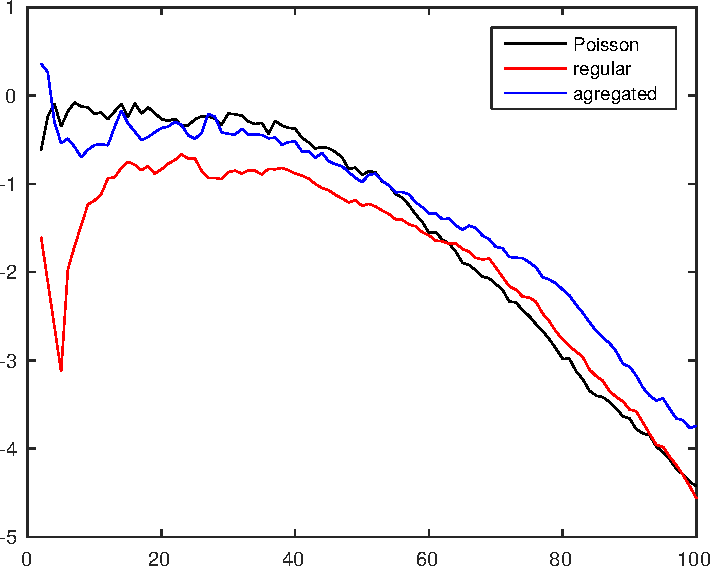
\includegraphics[width=10cm]{../matlab/ripley.pdf}
 \caption{Ripley's function $L(r)-r$.}
 \label{fig:point_process_generation:matlab:ripleyL}
\end{figure}
} 

\begin{figure}
 \centering
 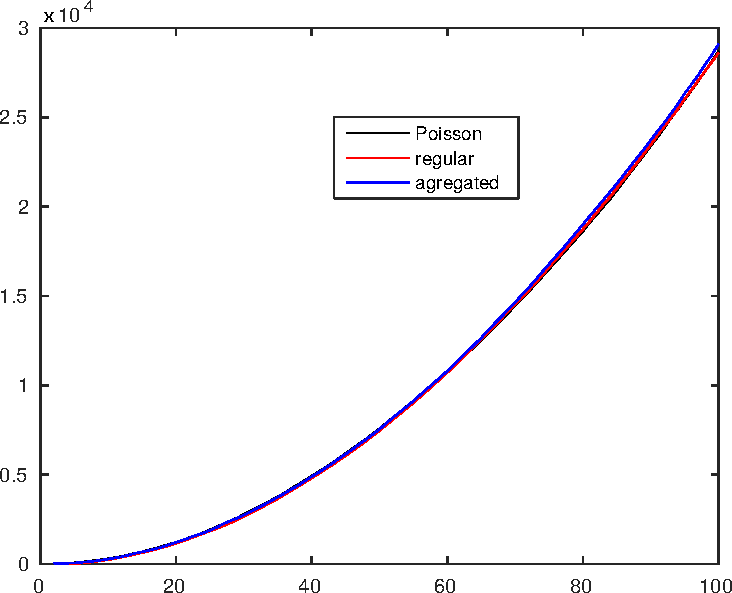
\includegraphics[width=10cm]{ripleyK.pdf}
 \caption{Ripley's K function for 3 different processes.}
 \label{fig:point_process_generation:matlab:ripleyK}
\end{figure}
 
\begin{matlab}
function [K, L, vals]=ripley(x,y,xmin,xmax,ymin,ymax,edges)
% Ripley K and L functions
% x and y define the points abscisses and ordinates
% xmin xmax ymin ymax define the domain
% edges is a vector containing the distances (typically, r=1:100 for example)
% K: K function
% L: L function
% vals: values of radius

% number of points
nb_points=length(x);

% area
area = (xmax-xmin)*(ymax-ymin);

% computes the distances between all pairs of points
d = pdist([x,y]);

h = histcounts(d, edges, 'Normalization', 'cumcount');

% count mean number of points
% multiply by 2 because each distance is only counted once in g
K = 2*h/nb_points;

% estimates density
densite=nb_points/area;
K=K/densite;

L = sqrt(K/pi);

vals = edges(1:end-1)+diff(edges);
end % of function
\end{matlab}

The code to generate these results is:
\begin{matlab}
r=1:100;
xmin=0; xmax=1000; ymin=0; ymax=1000;
nb_points=2000;
[x,y] = semi_alea(nb_points, xmin, xmax, ymin, ymax);
[k1,l1, vals]=ripley(x,y,xmin, xmax, ymin, ymax, r);

steps = [0,5,10];
energy= [10,0,0];
functionEnergy = @(x)stairsEnergy(x,steps, energy);
[x2,y2]=semis_inter(nb_points, xmin, xmax, ymin, ymax, 2000, functionEnergy);
[k2,l2, vals]=ripley(x2,y2, xmin, xmax, ymin, ymax, r);


steps = [0,2,5,10];
energy= [-10,10,0,0];
functionEnergy = @(x)stairsEnergy(x,steps, energy);
[x3,y3]=semis_inter(nb_points, xmin, xmax, ymin, ymax, 2000, functionEnergy);
[k3,l3, vals]=ripley(x3,y3, xmin, xmax, ymin, ymax, r);

% figures
figure
plot(vals,l1-vals,'k-');hold on;
plot(vals,l2-vals,'r-');hold on;
plot(vals,l3-vals,'b-');hold on;
legend('Poisson','regular','agregated');
title('Ripley L functions');

figure
plot(vals, k1, 'k-'); hold on
plot(vals, k2, 'r-'); 
plot(vals, k3, 'b-');

legend('Poisson','regular','agregated');
title('Ripley K function');
\end{matlab}


\subsection{Marked point process}
\begin{matlab}
figure
subplot(121)
% generates Poisson process
nb_points=50;
xmin=0;
xmax=100;
ymin=0;
ymax=100;
[x,y]=semi_alea(nb_points,xmin, xmax, ymin, ymax);
plot(x,y,'*');title('Poisson process');
axis square
axis([-20,120,-20,120]);

% Generates radii with mean mu and stddev sigma
sigma=1;
mu = 5;
r = sigma*randn(length(x), 1) + mu;

% generates plot with disks
subplot(122)
plot(x,y,'*'); 
hold on
theta=0:0.01:2*pi;
xx = zeros(length(theta), 1);
yy = xx;

% the second mark (color) can be generated as this
nb_colors = 10;
m2 = randi(nb_colors, nb_points, 1);
cmap =  hsv(nb_colors);

for i=1:length(x)
    xx=x(i)+r(i)*cos(theta);
    yy=y(i)+r(i)*sin(theta);
    plot(xx,yy,'LineWidth', 2, 'Color', cmap(m2(i),:));
end

axis square
axis([-20,120,-20,120]);
\end{matlab}

An example result is shown in \iflabelexists{fig:point_process_generation:circles}{Fig.\ref{fig:point_process_generation:circles}}
{Fig.\ref{fig:point_process_generation:matlab:circles}.

\begin{figure}[htbp]
 \centering
 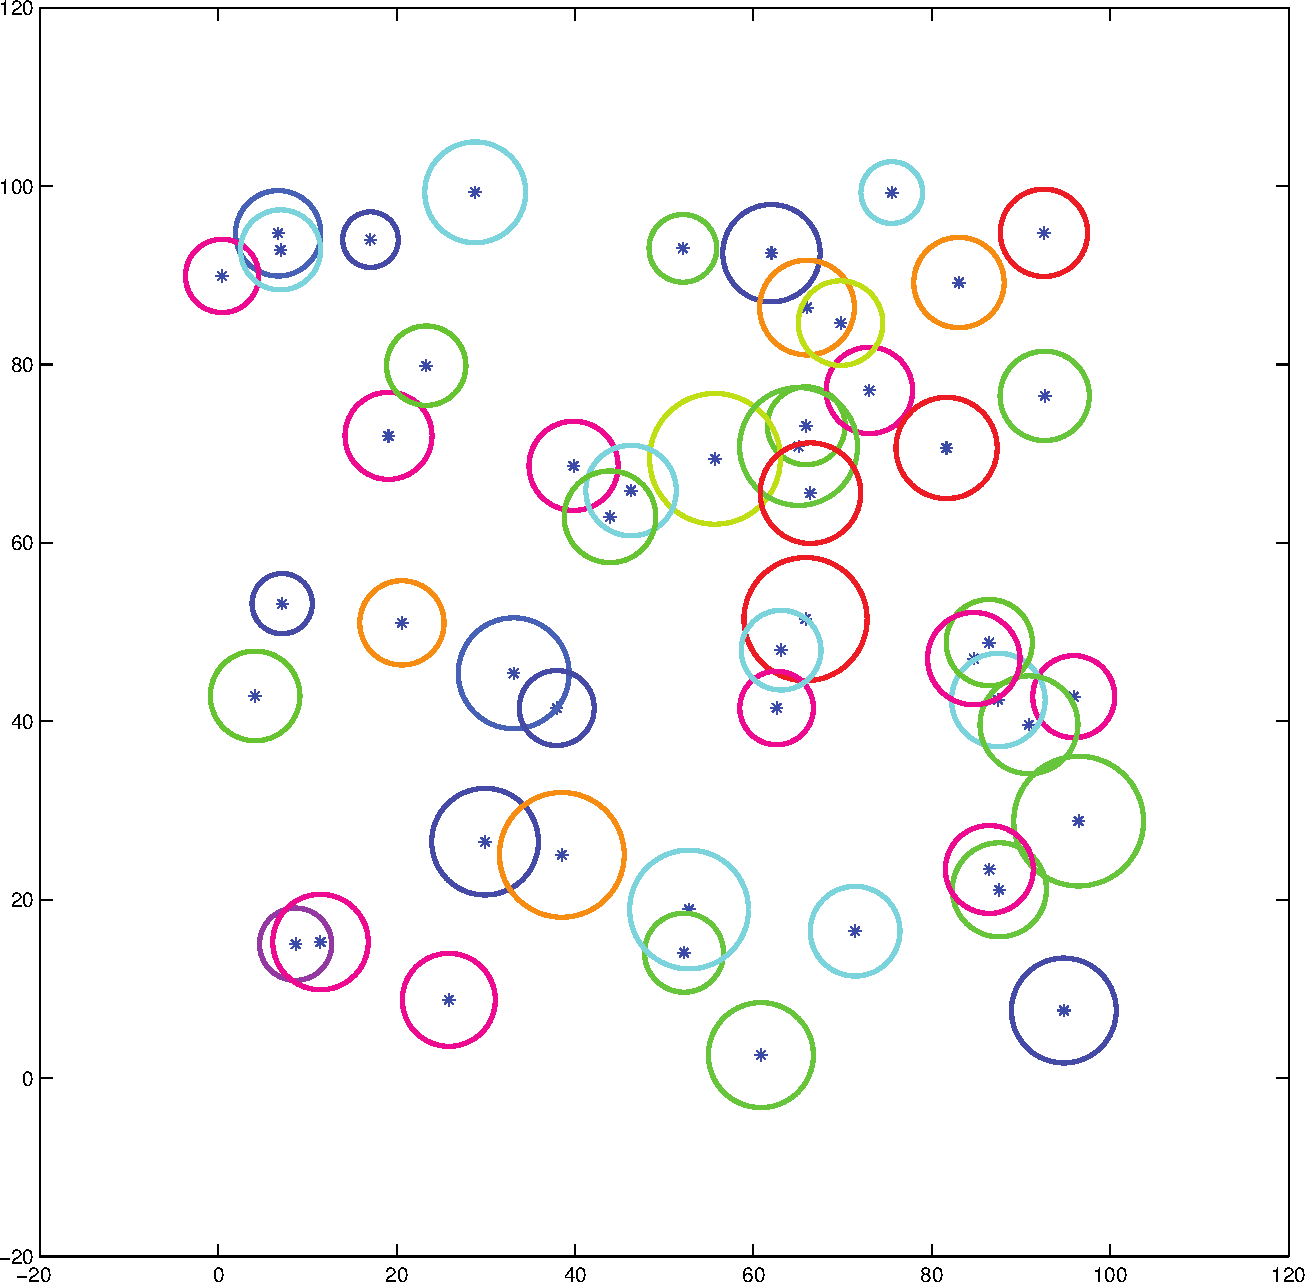
\includegraphics[width=6cm]{circles.pdf}
 \caption{A Poisson point process is used to generates the center of the circles. The radii are chosen according a Gaussian law, and the 
color according a uniform law.}
 \label{fig:point_process_generation:matlab:circles}
\end{figure}
}
